\documentclass[]{article}
\usepackage{graphicx}
\usepackage{amsmath}

%opening
\title{Chapter 02: Protocol Building Blocks}
\author{Uday Manchanda}

\begin{document}

\maketitle

\begin{abstract}
\centering{Chapter 02 Notes in the book \textit{Applied Cryptography} by Bruce Schneier}
\end{abstract}

\section{2.1: Introduction to Protocols}
\begin{itemize}
    \item Protocol: series of steps, involving two or more parties, designed to accomplish a task
    \item Everyone involved must know the protocol and all the steps involved
    \item Cryptographic protocol: protocol that uses cryptography
    \item The Purpose of Protocols
    \begin{itemize}
        \item Purpose is to prevent/detect eavesdropping and cheating
        \item \textbf{It should not be possible to do more or learn more than what is specified in the protocol}
        \item Protocols help to formalize how things are document
        \item Don't assume that everyone is honest; in-fact, it may be best to assume everyone is dishonest
    \end{itemize}
    \item The Players
    \begin{itemize}
        \item Alice + Bob are the two person protocols (Alice will initiate, Bob will respond)
        \item Carol + David for later roles
    \end{itemize}
    \item Arbitrated Protocols
    \begin{itemize}
        \item Arbitrator: disinterested third party trusted to complete a protocol
        \item He/she has no interested in the protocol and no particular allegiance to either party, all people involved trust this person
        \item 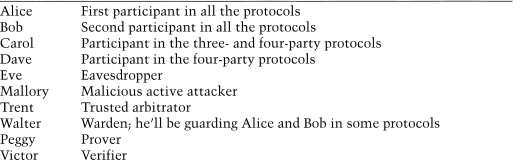
\includegraphics[width=0.5\textwidth]{people}
        \item In the real world, lawyers and bankers act as arbitrators
        \item Arbitrator can be the vulnerable point in the protocol as everyone must trust him and he/she musn't be a crook
    \end{itemize}
    \item Adjudicated Protocols
    \begin{itemize}
        \item Two types of arbitrated protocols
        \item Nonarbitrated protocol: the parties just want to complete the protocol
        \item Arbitrated protocol: if a dispute arises, an adjudicator comes in to determine if the protocol was performed fairly
        \item Not always necessary
    \end{itemize}
    \item Self Enforcing Protocol
    \begin{itemize}
        \item The best kind where the protocol itself guarantees fairness
    \end{itemize}
    \item Attacks against Protocols
    \begin{itemize}
        \item Passive attack: where someone not involved in the protocol can eavesdrop. He/she does not affect the protocol itself, but tries to gain info
        \item Active attack: someone tries to alter the protocol in their favor. This is far more serious
        \item The attacker could be one of the parties involved in the protocol. He/she is called a cheater. There are two types:
        \begin{itemize}
            \item Passive cheater: follows protocol, tries to obtain more information
            \item Active cheater: disrupt the protocol to their advantage
        \end{itemize}
    \end{itemize}
\end{itemize}
\section{2.2: Communications Using Symmetric Cryptography}
\begin{itemize}
    \item To communicate securely, encrypt communications
    \item For Alice to send an encrypted message to Bob
    \begin{itemize}
        \item Alice and Bob agree on a cryptosystem
        \item Alice and Bob agree on a key
        \item Alice takes her plaintext msg and encrypts it using the encryption algorithm and key. This creates a ciphertext message
        \item Alice sends ciphertext to Bob
        \item Bob decrypts the ciphertext message with the same algorithm and key reads it
    \end{itemize}
    \item A good cryptosystem is one in which all the security is inherent in knowledge of the key and none ins inherent in knowledge of the algorithm
    \item Hence why key management is so important
    \item The problems with symmetric cryptosystems
    \begin{itemize}
        \item Keys must be distributed in secret as key are as valuable as all of the messages they encrypt
        \item If a key is compromised, then an attacker (Eve) can decrypt all message traffic encrypted with that key
        \item If a separate key is used for each pair of users, the number of keys increases rapidly as the number of users goes uses
        \item Specifically, $\frac{n(n-1)}{2}$ keys are needed for a group of $n$ users
    \end{itemize}
\end{itemize}
\section{2.3: One-Way Functions}
\begin{itemize}
    \item A one-way function is a type of function where it is "easy" to compute but much more difficult to reverse
    \item Given $x$, one may calculate $f(x)$. But given $f(x)$, it is very difficult to compute $x$
    \item In a strictly mathematical sense, there is no evidence that one-way functions actually exist or even be constructed
    \item However, many cryptrographic functions are able to be computed easily but reversing them is nearly impossible
    \item A trapdoor one way function is a special type of one way function with a secret trapdoor
    \item It follows the same properties of a normal one way function; however, if you know the secret, you can easily compute the function in the other direction
\end{itemize}
\section{2.4: One-Way Hash Functions}
\begin{itemize}
    \item Hash function: takes variable length input (pre-image) and converts to a fixed length output (hash value)
    \item A simple hash function would be pre-image $\rightarrow$ byte consisting of all the XOR of all the input bytes
    \item Hash functions are many-to-one and works in one direction
    \item Should also be collision free; it is hard to generate two pre-images with the same hash value
    \item The actual hash functions are public, but their one-wayness is the real security
    \item Can be useful for verifying files: have the person send you the hash of the file
    \item If they match, the files are the same
    \item MAC: Message Authentication Code. A one way hash function with the addition of a secret key
    \item Hash value is the function of the pre-image and key
\end{itemize}
\section{2.5: Communications Using Public-Key Cryptography}
\begin{itemize}
    \item Symmetric algorithms are like safe where the key is the combination
    \item Public-key crytography involes two keys: one public and one private
    \item Computationally hard to deduce the private key from the public key
    \item Only the person with the private key can decrypt the message
    \item Public key crytography made it easier to send encrypted messages
    \item With symmetric encryption, both the sender and receiver needed to agree on a key
    \item Public key crypto is also easier to scale up
    \item Hybrid Cryptosystems
    \begin{itemize}
        \item Public key algorithms are used to encrypt keys not messages
        \item Therefore it is not a substitute for symmetric algorithms
        \item Two reasons for encrypting keys not messages
        \begin{itemize}
            \item 1. Public key algorithms are slow. Symmetric algorithms are 100x faster
            \item 2. Public key algorithms are vulnerable to chosen-plaintext attacks. 
            \item If $C=E(P)$ where P is one plaintext out of a set of n plaintexts, then a cryptanalyst only has to encrypt all n possible plaintexts and compare the results with C
            \item Encryption key is public
        \end{itemize}
        \item Chosen-plaintext attacks are effective if there are relatively few possible encrypted messages
        \item In most practical implementations P-K cryptography is used to secure and distribute session keys
        \item These session keys are then used with symmetric algorithms to secure message traffic
        \item Known as a hybrid cryptosystem
        \item Example of how it works
        \begin{itemize}
            \item Bob sends Alice his public key
            \item Alice generates a random session key, encrypts it using Bob's public key and sends to Bob
            \item Bob decrypts Alice's message using his private key to recover the sesion key
            \item Both of them encrypt their communications using the same session key
        \end{itemize}
        \item Session key is created when needed to encrypt communications and destroyed when no longer needed
        \item This makes it harder for an intruder to listen to messages
    \end{itemize}
    \item Merkle's Puzzles
    \begin{itemize}
        \item Ralph Merkle published a paper regarding Secure Communications over Insecure Channels
        \item His proposal was based on puzzles that were easier to solve for the sender and receiver than for an eavesdropper
        \item Alice can send an encrypted message to Bob without having to exchange a key
        \begin{itemize}
            \item Bob generates $2^{30}$ (~million) messages of the form: \textit{This is puzzle number x. This is the secret key number y}
            \item x is a random number, y is a random secret key; different for each message
            \item Using a symmetric algorithm he encrypts each message with a different 20bit key and sends them to Alice
            \item Alice chooses one message at random and performs a brute force attack to recover the plaintext. A very large task
            \item Alice encrypts her secret message with the key she recovered and some symmetric algorithm and sends to Bob along with x
            \item Bob knows which secret key y he encrypts in message x so he can decrypt the message
        \end{itemize}
        \item Eve (the eavesdropper) can break this system but has to do far more work
        \item To recover the message she has to perform a brute force attack against each of Bob's $2^{30}$ messages. Complexity of $2^{40}$
    \end{itemize}
\end{itemize}
\section{2.6: Digital Signatures}
\begin{itemize}
    \item Need a way to prove authorship
    \item Signing documents with physical signatures is not secure because they can be forged or copied easily
    \item Signing documents with Symmetric Cryptosystems and an Arbitrator
    \begin{itemize}
        \item Alice wants to sign digital message and send it to Bob
        \item she can do it with the help of Trent, a trusted arbitator, and a symmetric cryptosystem
        \item What happens:
        \begin{itemize}
            \item Alice encrypts message to Bob $K_{A}$ and sends to Trent
            \item Trent decrypts message with $K_{A}$
            \item Trent takes decrypted message and a statement that he has received this message from Alice and encrypts the whole bundle with $K_{B}$
            \item Trent sends the encrypted bundle to Bob
            \item Bob decrypts the bundle with $K_{B}$. He can read the message and Trent's certification that Alice sent it
        \end{itemize}
        \item Trent knows the message is from Alice because he infers from the message's encryption and because only they share the secret key
        \item However the arbitrator (Trent) acts as a bottleneck because every time Alice wants to send a message to Bob, she must send it via Trent first
        \item Also Trent must be perfect, even a slight error will render all the signatures he verified to be useless
    \end{itemize}
    \item Digital Signature Trees
    \begin{itemize}
        \item Uses a tree structure to produce an infinite number of one time signatures
        \item Place the root of the tree in a public file, thereby authenticating it
        \item Root signs one message and authenticates its sub nodes in the tree
        \item Each node then signs one message and authenticates its sub nodes, and so on
    \end{itemize}
    \item Signing Documents with PK Cryptography
\end{itemize}
\end{document}